\section{Spektroskopie der Hyperfeinstruktur von Rubidium}
\subsection{Durchführung}
\subsubsection*{Bestimmung der Scanrate des Lasers}
Zur Bestimmung der Stromabhängigkeit der
Laserfrequenz wird das Etalon in den Strahlengang eingesetzt und der Diodenstrom mit einem Dreiecksignal moduliert.
Der Konstantanteil des Laserstroms beträgt bei der Messung 64.7\,mA,
die Temperatur der Laserdiode 34.0$^\circ$C.
Die Modulation des Laserstroms findet mit dem \emph{instec function~generator} statt,
da dieser eine bessere Signalqualität als das Netzgerät des Versuchsaufbaus liefert.
Die Frequenz des Modulationssignals beträgt 0.1\,kHz, seine Amplitude 0.7\,V.

\subsubsection*{Vermessung der Hyperfeinstruktur-Übergänge}
Bei der Messung des Hyperfein-Absorptionsspektrums befinden sich die beiden Linsen und
die Rubidiumzelle im Strahlengang.
Der Konstantanteil des Laserstroms, Modulationsamplitude und -frequenz
sind wie bei der Messung der Zeitabhängigkeit der Laserfrequenz, um die dort bestimmte Scanrate
zur Auswertung der Messungen verwenden zu können.
Äußere Magnetfelder bleiben unkompensiert, weil die Zeeman-Aufspaltung der Hyperfeinstruktur im Erdmagnetfeld
mit der Linienbreite der Laserdiode nicht auflösbar ist.
Die Messung wird auf der steigenden und der fallenden Flanke der Modulationsspannung durchgeführt und
während der Messung wird die Zelle mit dem Föhn geheizt.

\subsection{Auswertung}
Die Auswertung wird beispielhaft für die Messung auf der steigenden Flanke beschrieben. Die Auswertung der fallenden Flanke erfolgt analog. 
Die Vorstellung der Ergebnisse und Diskussion erfolgt für beide Flanken.
\subsubsection*{Bestimmung der Scanrate des Lasers}
\label{sub:scanrate}
Das Etalonspektrum und die Spannung der Lasermodulation sind in \autoref{img:etalon:fit} dargestellt.
Die Peaks des Etalonspektrums werden mit Cauchy-Kurven und einem linearen Untergrund gefittet:
\begin{equation}
    U_\text{ph}(t) = a_\text{ph} + b_\text{ph} \cdot t + \frac{A}{\pi} \frac{s}{s^2 + (t-x)^2} \ \, .
\end{equation}
Dabei ist das Zentrum $x$ und der Breiteparameter $s$.
Des Weiteren wird die Spannung für die Lasermodulation $U_\text{L}$ mit einer Geraden gefittet.
\begin{equation}
    U_\text{L}(t) = a_\text{L} + b_\text{L} \cdot t
\end{equation}
\begin{figure}[H]
\begin{center}
    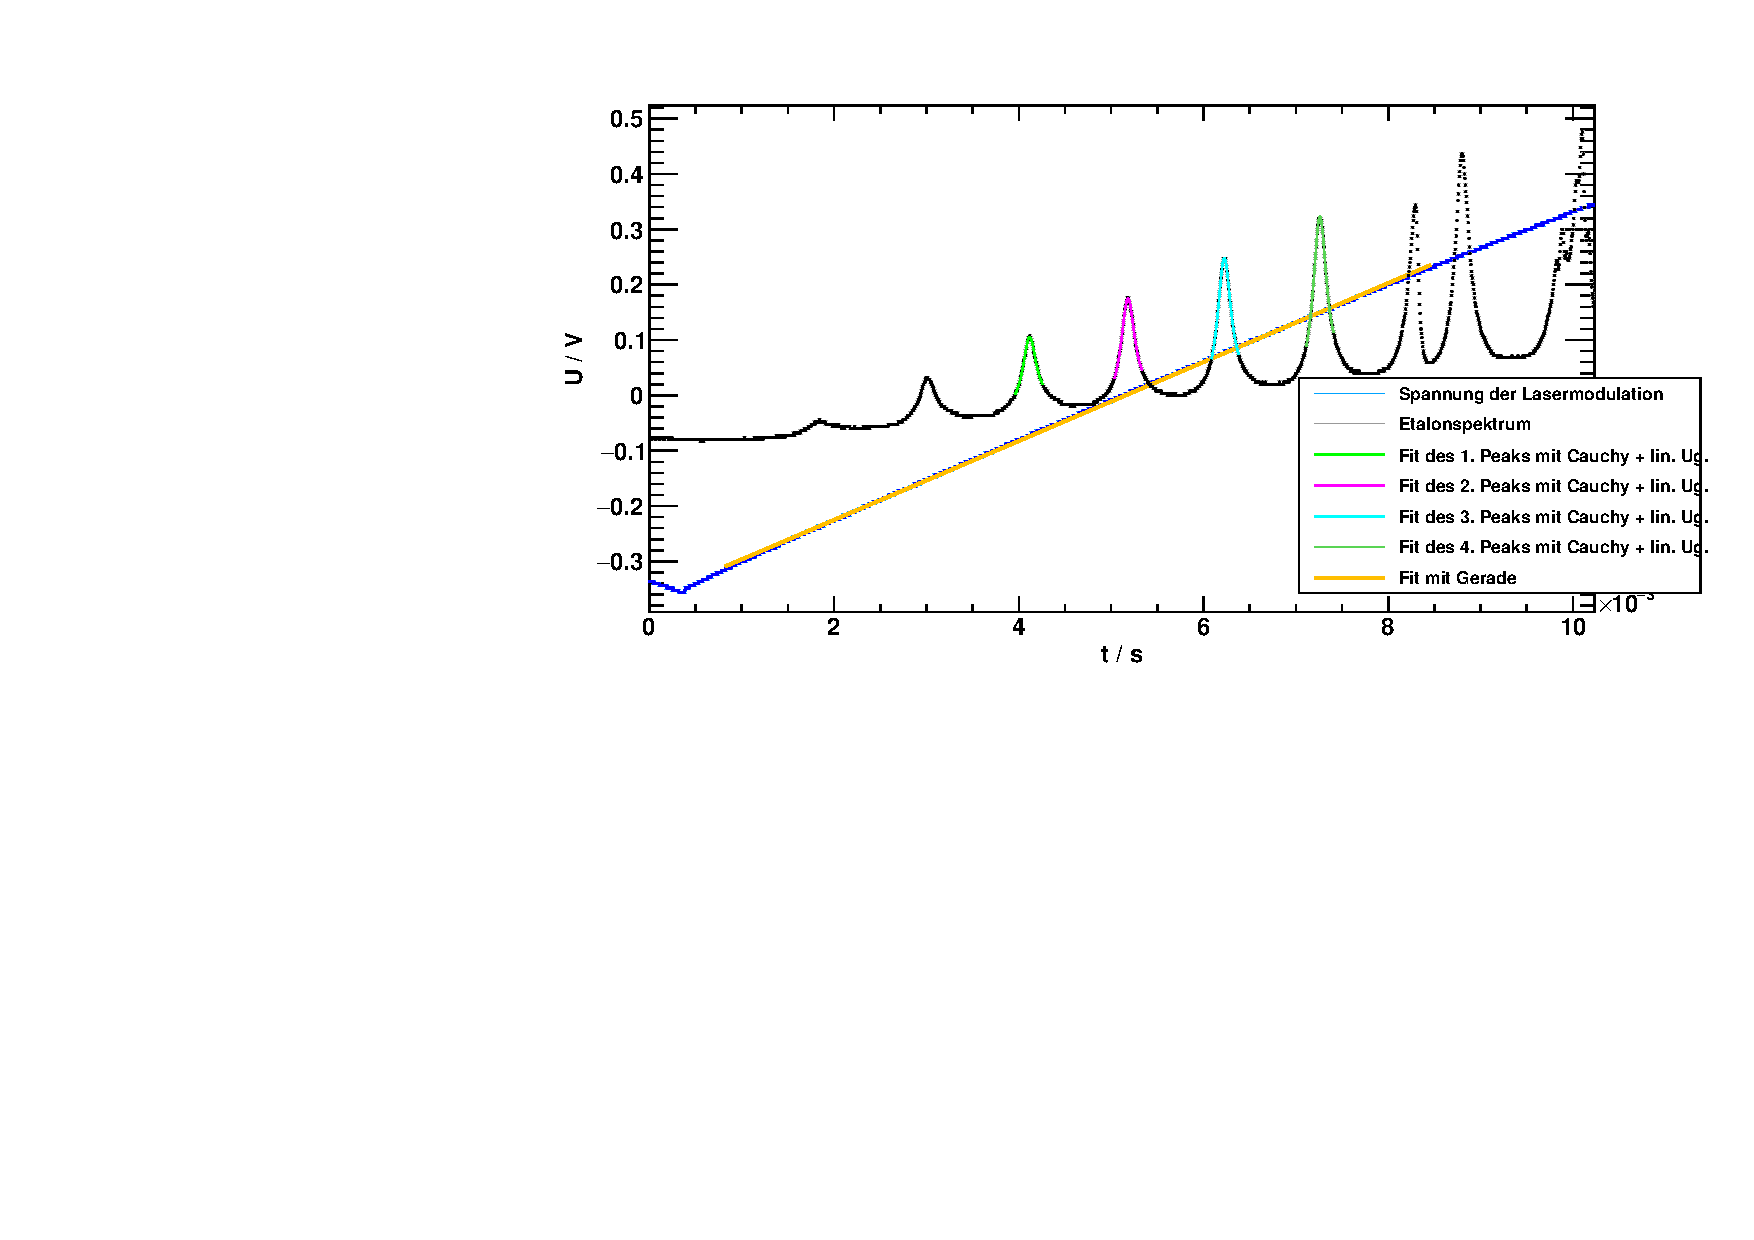
\includegraphics[width=\textwidth]{../img/part2/up-etalon_zoom_fit.pdf}
    \caption{Etalonspektrum mit Kurvenanpassungen der Peaks und
    Spannung für die Lasermodulation mit linearer Regression der Messung.
    Im rechten Bereich der Abbildung ist ein Modensprung erkennbar,
    die Messung des Hyperfeinspektrums findet daher zwischen 2. und 4. Etalonpeak statt.}
    \label{img:etalon:fit}
\end{center}
\end{figure}
Der Fit von $U_\text{L}$ kontrolliert, ob die Spannung für die Lasermodulation auch gerade ansteigt. Man erkennt, dass die angepasste Gerade 
im relevanten Zeitintervall gut der gemessenen Spannung folgt. Das reduzierte \textchi$^2$ beträgt 1.6. \\
Aus dem freien Spektralbereich des Etalons $\Delta \nu_\text{FSR} = (9924 \pm 30)\,\text{MHz}$ lässt sich nun die Differenz der Laserfrequenz von den verschiedenen
Peaks bestimmen. Der erste Peak wird als Referenzpeak festgelegt. Der Frequenzabstand $\nu_i$ zwischen erstem und $i$-tem Peak lässt sich nun
folgendermaßen berechnen\footnote{Gedankenspiel zur Fehlerrechnung: Interpretiert man $2 \cdot a$ als $a + a$, so ist der Fehler im ersten Fall $2 \cdot s_a$, im zweiten
allerdings $\sqrt{2} \cdot s_a$, wenn man die Selbstkorrelation von $a$ nicht berücksichtigt. Mit $\cor(a, a) = 1$
erhält man $\sqrt{s_a^2 + s_a^2 + 2 \cdot s_a \cdot s_a \cdot \cor(a, a)} = 2 \cdot s_a$.}:
\begin{equation}
    \Delta \nu_i = i \cdot \Delta \nu_\text{FSR}, \qquad s_{\Delta \nu_i} = i \cdot s_{\Delta \nu_\text{FSR}}
\end{equation}
Die Frequenzabstände $\Delta \nu_i$ werden nun gegen die Zentren $x_i$  der
Etalonpeaks aufgetragen (\autoref{img:etalon:calibration}). Da die Fehler auf die Zentren der Cauchy-Funktionen sehr klein sind, werden die Fehler 
auf $\frac{1}{5}$ der Breiteparameter $s_i$ gesetzt. Die so berechneten Werte sind in \autoref{tab:etalon:calib:up} aufgelistet.
\begin{table}[H]
\caption{Zentren $x_i$ der gefitteten Cauchy-Funktionen mit abgeschätztem Fehler aus den Breiteparametern $s_i$ und Frequenzdifferenzen zum ersten Peak. }
\begin{center}
\begin{tabular}{|c|c|c|c|c|}
  \hline
  i & $x_i$ / s & $0.2 \cdot s_i$ / s & $\nu_i$ / GHz & $s_{\nu_i}$ / GHz \\ \hline
  1 & 4.117 & 0.018 & 0.00 & 0.00 \\ \hline
  2 & 5.181 & 0.018 & 9.92 & 0.03 \\ \hline
  3 & 6.225 & 0.018 & 19.85 & 0.06 \\ \hline
  4 & 7.260 & 0.018 & 29.77 & 0.09 \\ \hline
\end{tabular}
\end{center}
\label{tab:etalon:calib:up}
\end{table}

\begin{figure}[H]
\begin{center}
    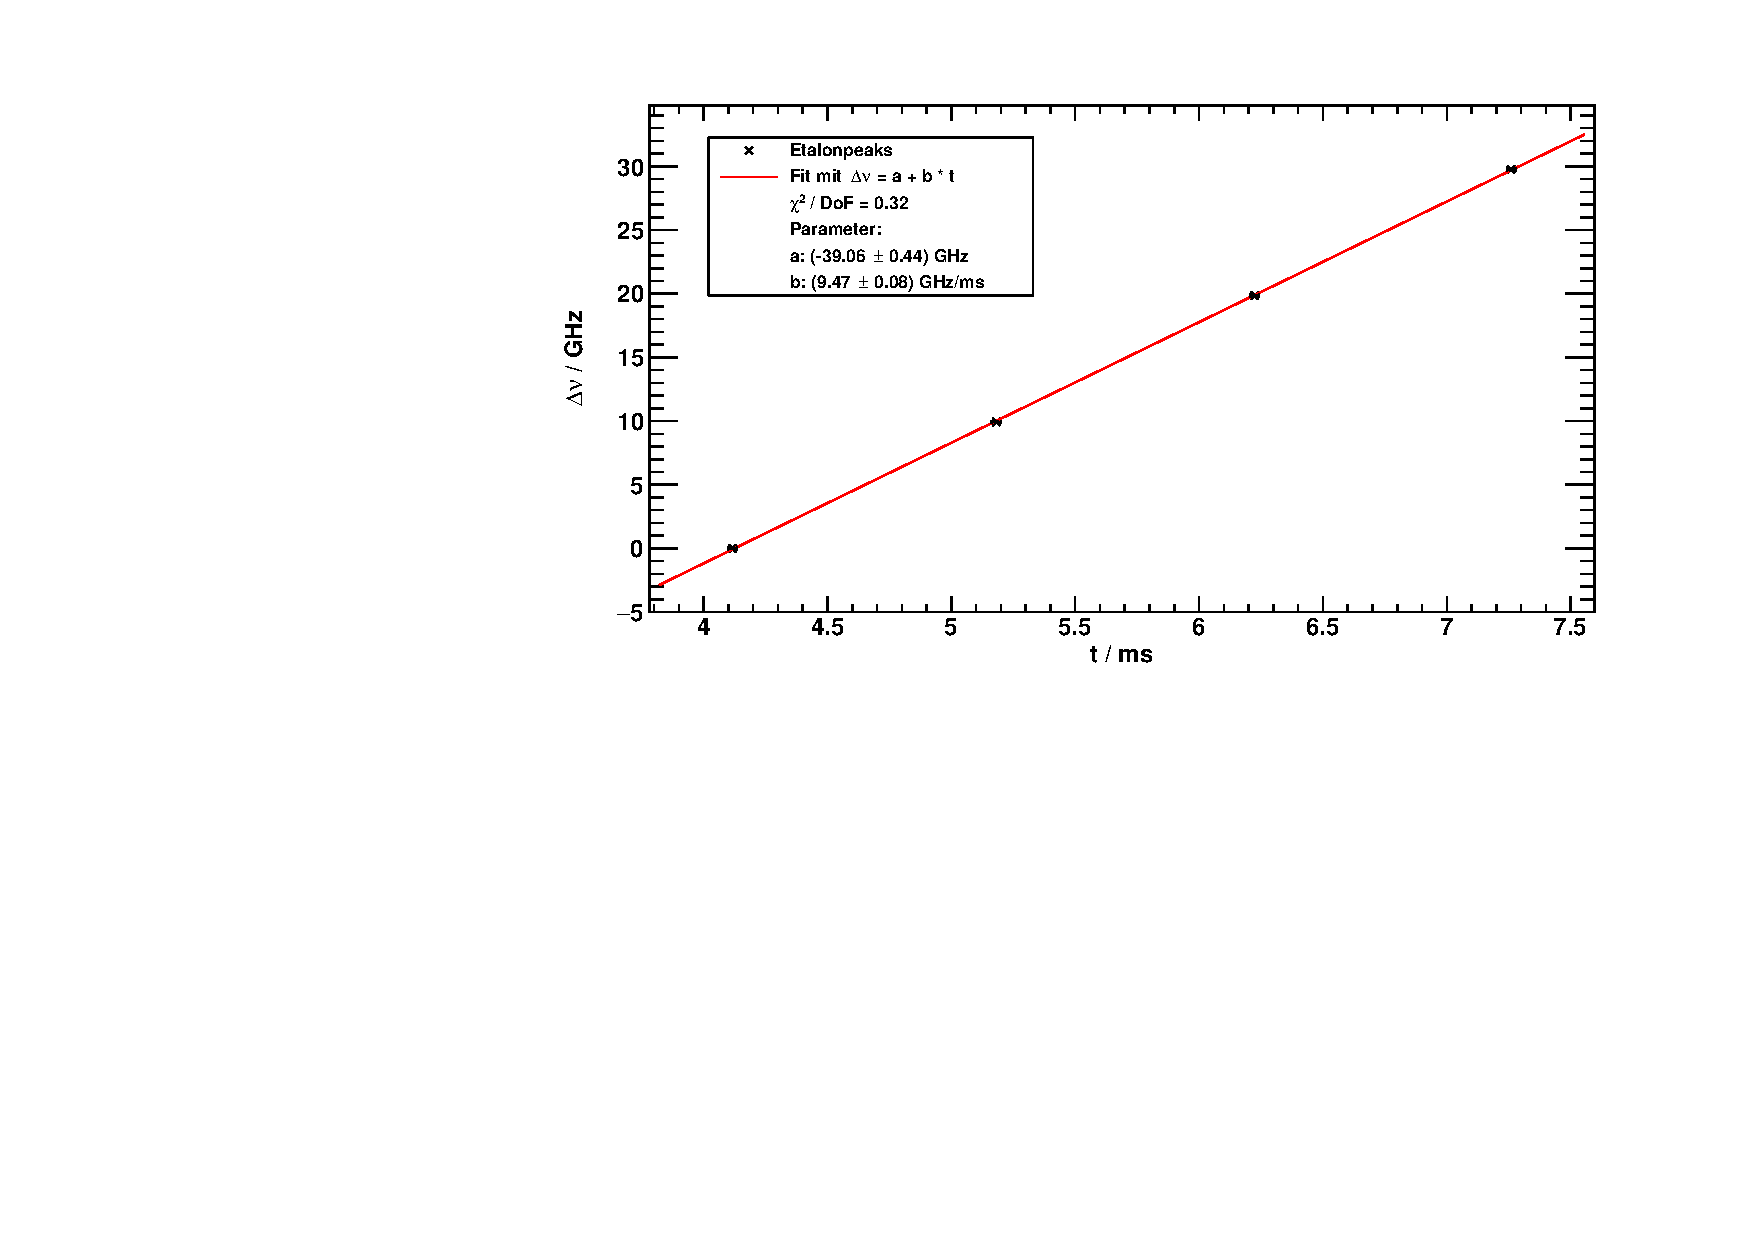
\includegraphics[width=\textwidth]{../img/part2/up-etalon_zoom-etalon_calibration.pdf}
    \caption{Frequenzdifferenz der Etalonpeaks aufgetragen gegen ihre Positionen. Bestimmung der Laserscanrate durch linearen Fit.}
    \label{img:etalon:calibration}
\end{center}
\end{figure}
Aus dem Fit mit einer Geraden
\begin{equation}
    \Delta \nu(t) = a + r \cdot t 
\end{equation}
lässt sich nun die Scanrate $r$ bestimmen, mit welcher die Frequenz des Lasers pro Zeit geändert wird. Man erhält
\begin{equation}
    r = (9.47 \pm 0.08)\,\frac{\text{GHz}}{\text{ms}}\ \, .
\end{equation}

\subsubsection*{Hyperfeinstruktur-Übergänge}
Auf dem aufgenommenen Spektrum (\autoref{img:hfs:fit:up}) der Hyperfeinstruktur von Rubidium sind nur sechs der acht erwarteten
Übergänge zu erkennen (vgl. \autoref{img:hfsspectrum}). Dies liegt daran, dass je zwei Übergänge so dicht beieinander liegen,  %TODO Ref Grundlagen
dass man sie in diesem Versuchsaufbau nicht mehr
einzeln auflösen kann. Für die gut abtrennbaren Gruppen von
mehreren Peaks der Übergänge werden überlagerte Gauß-Funktionen mit einem linearen Untergrund zur Kurvenanpassung verwendet:
\begin{equation}
    \begin{split}
        & \gaus(x; A, \mu, \sigma) := A \cdot e^{-\frac{1}{2} \left( \frac{x-\mu}{\sigma} \right)^2} \\
        & U_\text{ph}(t) = a + b \cdot t + \sum_{i=1}^N \gaus(t; A_i, \mu_i, \sigma_i)
    \end{split}
\end{equation}
$N$ gibt an, wie viele Peaks sich überlagern.
\begin{figure}[H]
\begin{center}
    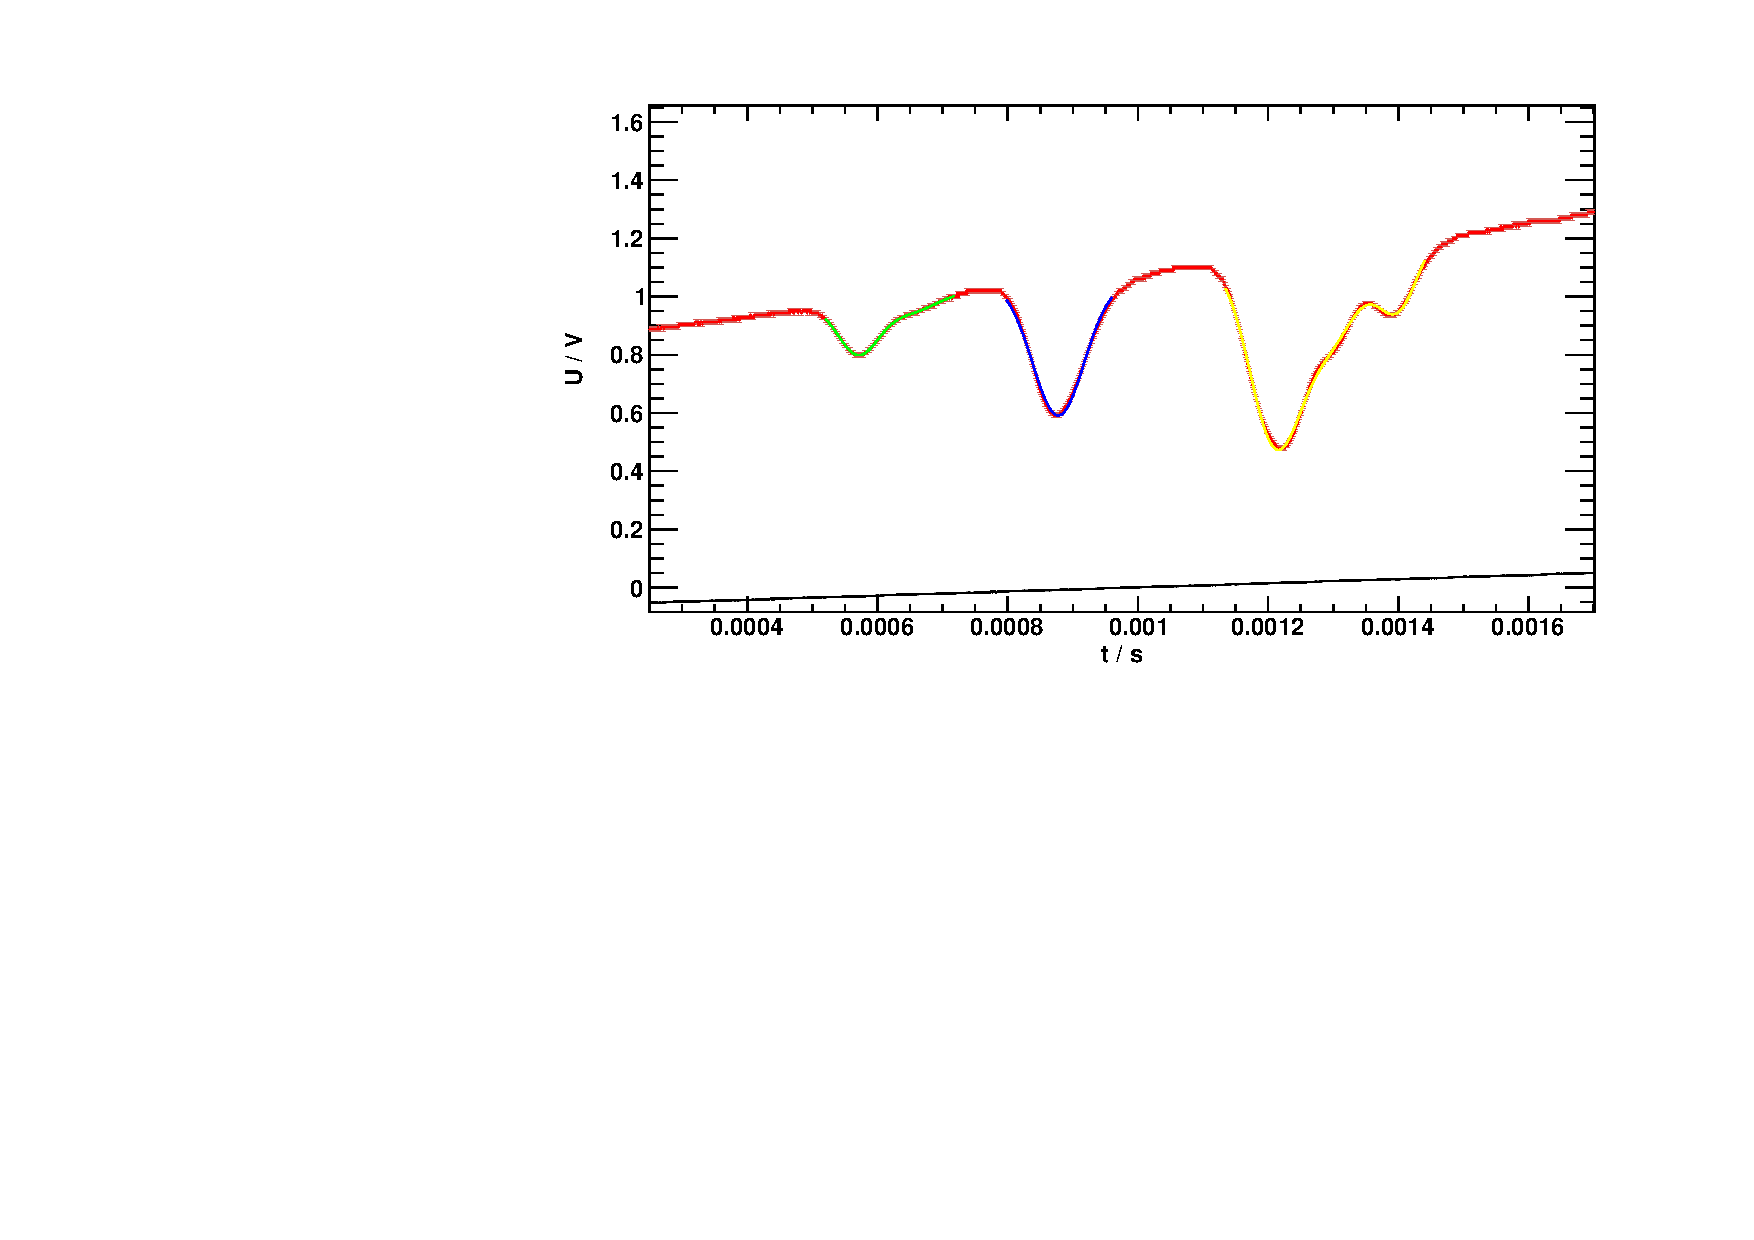
\includegraphics[width=\textwidth]{../img/part2/up-hfs_zoom_fit.pdf}
    \caption{Hyperfeinstrukturspektrum von Rubidium mit Fits der sich teilweise überlagernden Peaks.}
    \label{img:hfs:fit:up}
\end{center}
\end{figure}
In \autoref{tab:hfs:peaks:up} sind die Erwartungswerte $\mu_i$ und Standardabweichungen $\sigma_i$ der gefitteten Gauß-Funktionen aufgelistet. 
Da auch hier der Fehler auf die Erwartungswerte sehr klein ist, wird der Fehler auf $\frac{1}{5}$ der Standardabweichung gesetzt.
\begin{table}[H]
\caption{Erwartungswerte $\mu_i$ und Standardabweichungen $\sigma_i$ der gefitteten Peaks des HFS-Spektrums.}
\begin{center}
\begin{tabular}{|c|c|c|c|c|}
  \hline
  Peak $i$ & $\mu_i$ / ms & $s_{\mu_i}$ / ms & $\sigma_i$ / \textmu s & $s_{\sigma_i}$ / \textmu s \\ \hline
  1 & 0.57072 & 0.00103 & 31.4 & 1.2 \\ \hline
  2 & 0.65033 & 0.01409 & 39.7 & 6.4 \\ \hline
  3 & 0.87686 & 0.00007 & 37.0 & 0.4 \\ \hline
  4 & 1.21876 & 0.00009 & 53.2 & 0.6 \\ \hline
  5 & 1.30931 & 0.00022 & 23.7 & 0.3 \\ \hline
  6 & 1.38975 & 0.00024 & 43.5 & 0.9 \\ \hline
\end{tabular}
\end{center}
\label{tab:hfs:peaks:up}
\end{table}


\subsubsection*{Berechnung des Spektrums}
Da die Differenzen der einzelnen Hyperfeinniveaus in der Größenordnung von $10^9$\,Hz liegen und die absoluten Frequenzen bei $10^{14}$\,Hz, 
wird darauf verzichtet, die absoluten Frequenzen auszurechnen. Der Peak mit der größten Amplitude (Peak 4) wird als Referenz gesetzt. Von ihm aus werden 
die Differenzen zu den anderen Peaks berechnet. Dazu wird die oben (\autoref{sub:scanrate}) berechnete Scanrate $r$ des Lasers benötigt.
Die Differenzen der Frequenzen $\Delta \nu_i$ zwischen viertem und $i$-tem Peak berechnen sich nun mit
\begin{equation}
    \Delta \nu_i = r \cdot \left( \mu_i - \mu_4 \right), 
    \qquad s_{\Delta \nu_i} = \Delta \nu_i \sqrt{ \left( \frac{s_r}{r} \right)^2 + \frac{s_{\mu_i}^2 + s_{\mu_4}^2}{ \left( \mu_i - \mu_4 \right)^2 }} \ \, .
\end{equation}
Mit dieser Formel für den Fehler von $\Delta \nu_i$ ist der Fehler auf $\Delta \nu_4$ nicht definiert, da eine Division durch Null stattfindet.
Um doch einen Fehler zu bekommen, wird hier angenommen, dass $\mu_4$ (des Referenzpeaks) keinen Fehler hat. Man erhält mit Gauß'scher Fehlerfortpflanzung
\begin{equation}
    s_{\Delta \nu_4} = r \cdot s_{\mu_4} \ \, .
\end{equation}
Um die theoretischen Werte sinnvoll mit den gemessenen Werten zu vergleichen, müssen die theoretischen Differenzen der Frequenz den gleichen 
Übergang als Referenz benutzen. Dies erreicht man, wenn die Differenz der Frequenz des Referenzübergangs von allen Differenzen abgezogen wird.
In \autoref{tab:hfs:spectrum} sind die theoretischen (\autoref{img:hfsspectrum}) und (für steigende und fallende Flanke) experimentell bestimmten Spektren aufgelistet.   
\begin{table}[H]
\caption{Theoretisches und experimentell bestimmtes (steigende und fallende Flanke) Hyperfeinstrukturspektrum von Rubidium.}
\begin{center}
\begin{tabular}{|c|c|c|c|c|c|}
  \hline
  Übergang & $\Delta \nu^\text{theo}$ / GHz & $\Delta \nu^\text{exp}_\text{up}$ / GHz & $s_{\Delta \nu^\text{exp}_\text{up}}$ / GHz & $\Delta \nu^\text{exp}_\text{down}$ / GHz & $s_{\Delta \nu^\text{exp}_\text{down}}$ / GHz \\ \hline
  \rb{87}, F:2-1 & -4.81 & -4.86 & 0.12 & -4.95 & 0.10 \\ \hline
  \rb{87}, F:2-2 & -3.99 & -4.10 & 0.09 & -4.24 & 0.10 \\ \hline
  \rb{85}, F:3-2, 3-3 & -3.04 & -3.24 & 0.13 & -3.25 & 0.12 \\ \hline
  \rb{85}, F:2-2, 2-3 & 0.00 & 0.00 & 0.07 & -0.00 & 0.07 \\ \hline
  \rb{87}, F:1-1 & 2.02 & 2.15 & 0.10 & 2.01 & 0.09 \\ \hline
  \rb{87}, F:1-2 & 2.84 & 2.90 & 0.09 & 2.85 & 0.10 \\ \hline
\end{tabular}
\end{center}
\label{tab:hfs:spectrum}
\end{table}

Zur Überprüfung, wie gut die theoretischen Daten mit den Gemessenen übereinstimmen, werden sie gegeneinander aufgetragen 
(\autoref{img:hfs:spectrum:up} für die steigende und \autoref{img:hfs:spectrum:down} für die fallende Flanke). Es sollte sich 
eine Gerade mit Steigung 1 und Achsenabschnitt 0 ergeben.

\begin{figure}[H]
\begin{center}
    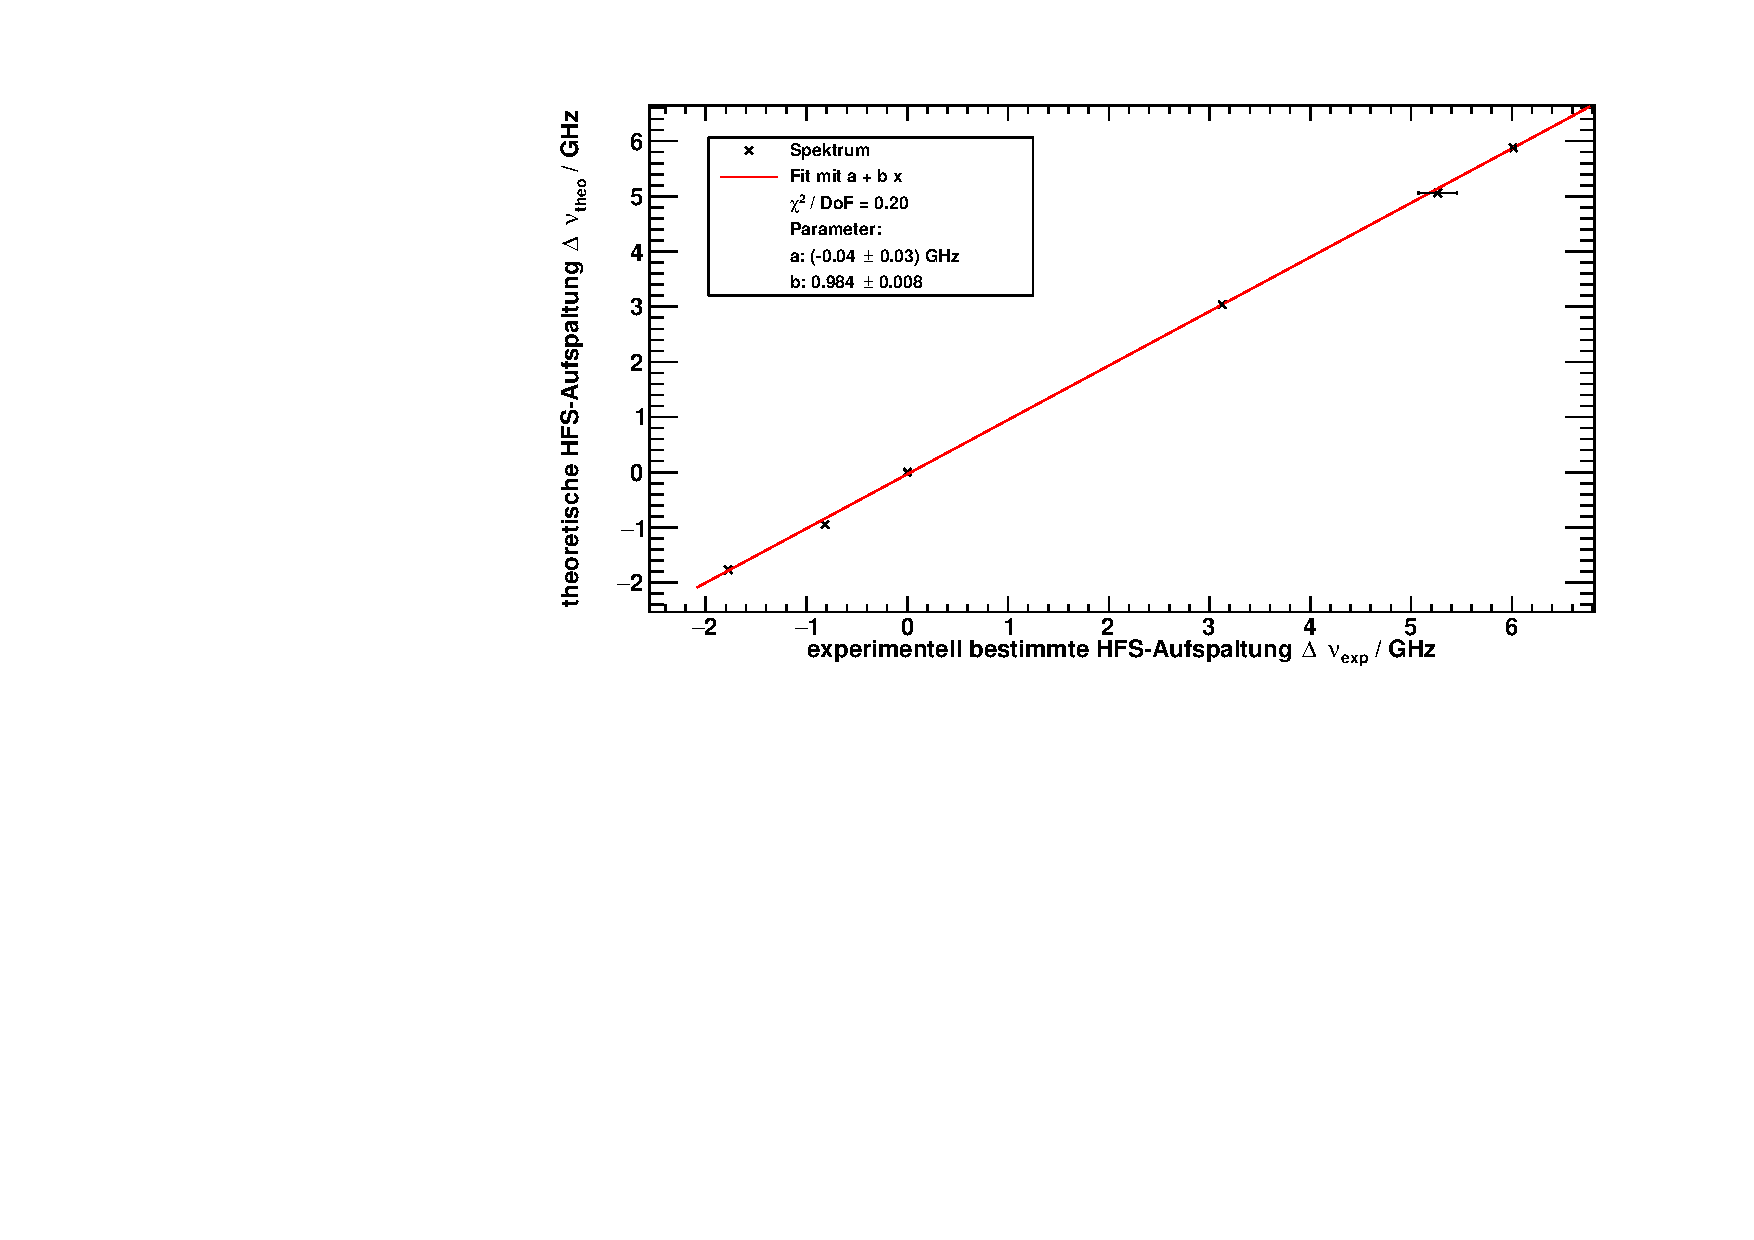
\includegraphics[width=\textwidth]{../img/part2/up-spectrum.pdf}
    \caption{Vergleich des auf der steigenden Flanke gemessenen Hyperfeinstrukturspektrums mit den theoretischen Werten.}
    \label{img:hfs:spectrum:up}
\end{center}
\end{figure}

\begin{figure}[H]
\begin{center}
    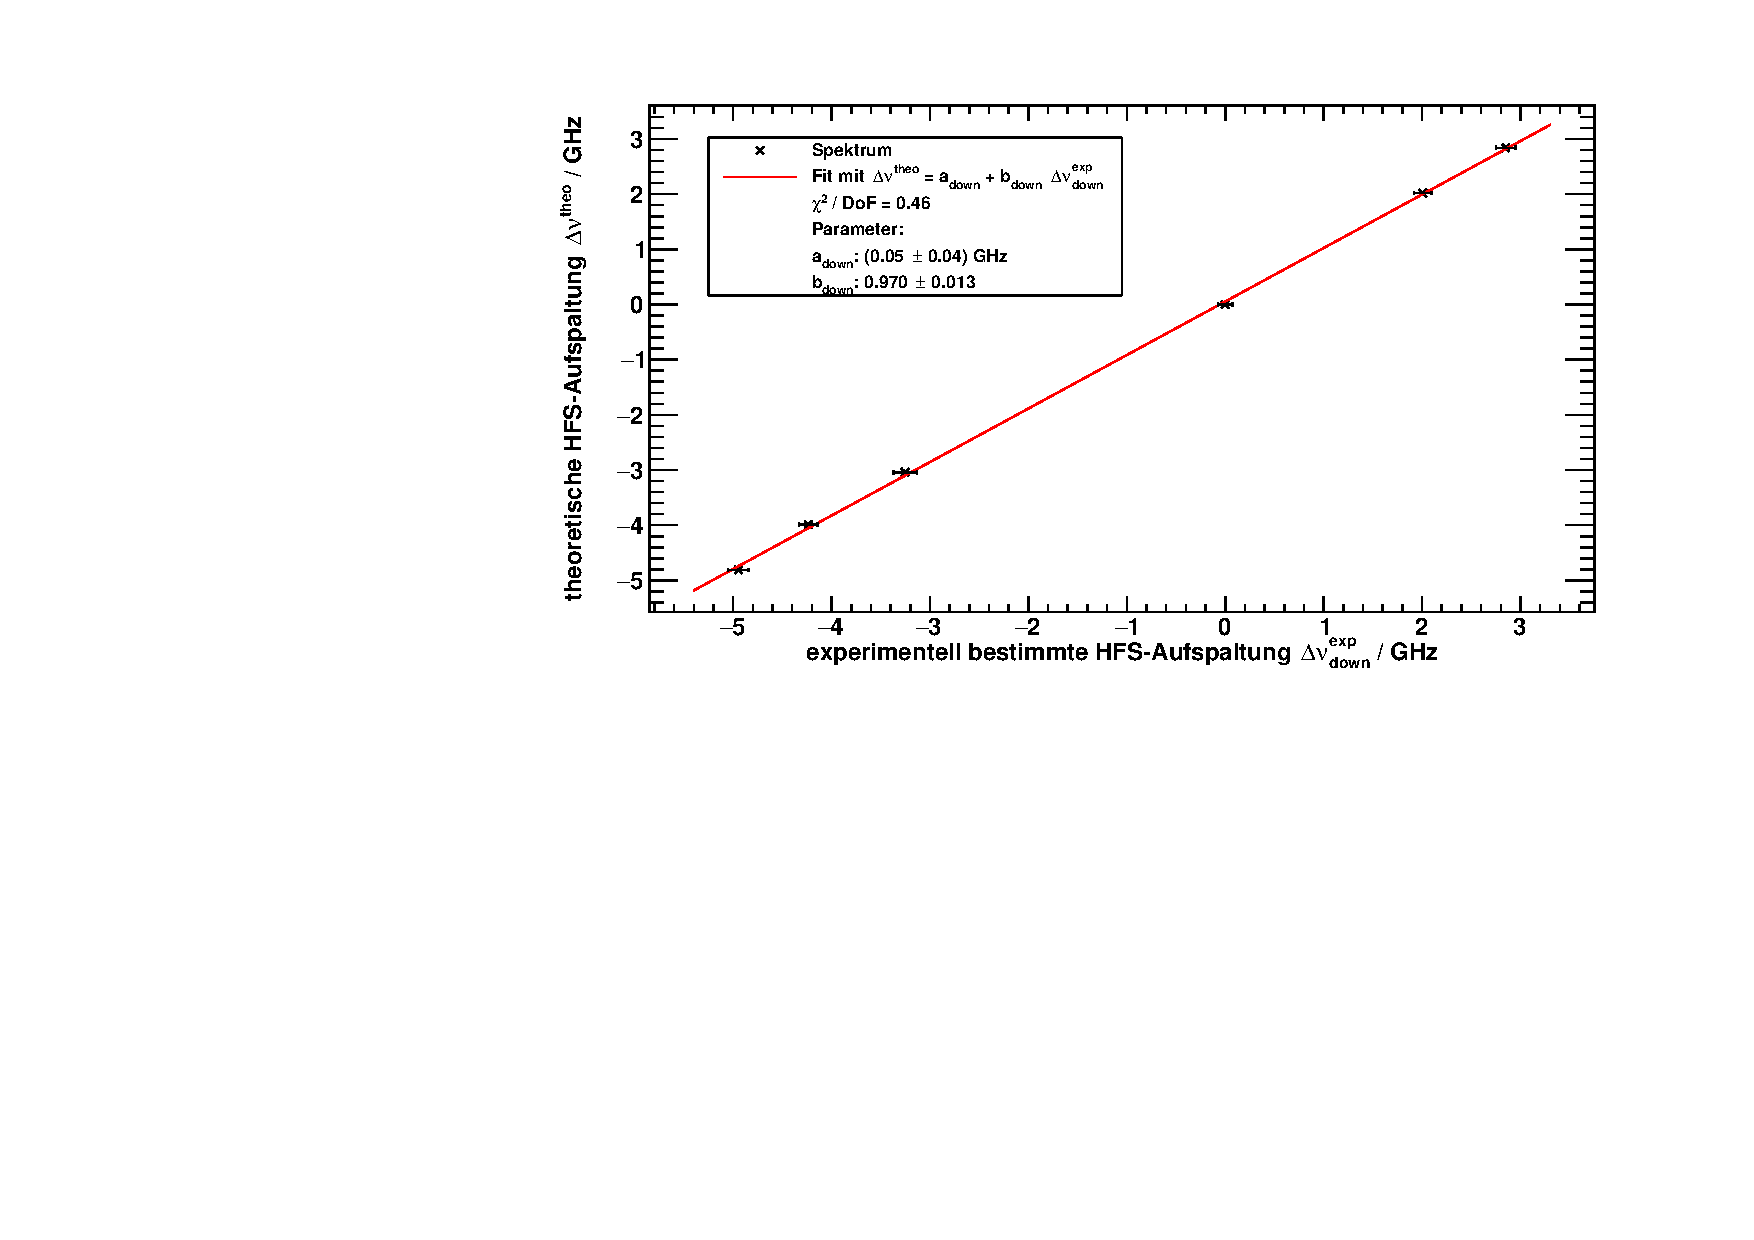
\includegraphics[width=\textwidth]{../img/part2/down-spectrum.pdf}
    \caption{Vergleich des auf der fallenden Flanke gemessenen Hyperfeinstrukturspektrums mit den theoretischen Werten.}
    \label{img:hfs:spectrum:down}
\end{center}
\end{figure}
Die Achsenabschnitte 
\begin{equation}
    a_\text{up} = (-0.01 \pm 0.04)\,\text{GHz} \quad \text{und} \quad a_\text{down} = (0.05 \pm 0.04)\,\text{GHz}
\end{equation}
sind wie erwartet verschwindend.
Die Steigungen
\begin{equation}
    b_\text{up} = (0.973 \pm 0.013) \quad \text{und} \quad b_\text{down} = (0.970 \pm 0.013)
\end{equation}
sind innerhalb des 3-\textsigma-Intervalls gleich 1. Da die beiden beiden Werte untereinander gut übereinstimmen, gehen wir von einem systematischen 
Fehler bei den Messungen aus. Zum Beispiel könnte das Etalon im Strahlengang verkippt gewesen sein, was zur Verkleinerung des freien Spektralbereichs führt. 
Dadurch vergrößern sich die Peakabstände der experimentell bestimmten Spektren und die Steigung der Geraden nimmt ab.

\subsubsection*{Berechnung der Intervallkonstanten $A$}
Für die Berechnung der Intervallkonstanten $A$ wird für jeden Übergang das gewichtete Mittel der Abstände vom Referenzpeak 
von steigender und fallender Flanke gebildet (\autoref{tab:hfs:spectrum:avg}).
\begin{table}[H]
\caption{Theoretisches und aus den experimentellen Daten gemitteltes Hyperfeinstrukturspektrum von Rubidium.}
\begin{center}
\begin{tabular}{|c|c|c|c|}
  \hline
  Übergang & $\Delta \nu^\text{theo}$ / GHz & $\Delta \nu^\text{exp}_\text{avg}$ / GHz & $s_{\Delta \nu^\text{exp}_\text{avg}}$ / GHz \\ \hline
  \rb{87}, F:2-1 & -4.81 & -4.907 & 0.077 \\ \hline
  \rb{87}, F:2-2 & -3.99 & -4.162 & 0.065 \\ \hline
  \rb{85}, F:3-2, 3-3 & -3.04 & -3.246 & 0.087 \\ \hline
  \rb{85}, F:2-2, 2-3 & 0.00 & 0.000 & 0.051 \\ \hline
  \rb{87}, F:1-1 & 2.02 & 2.065 & 0.067 \\ \hline
  \rb{87}, F:1-2 & 2.84 & 2.876 & 0.069 \\ \hline
\end{tabular}
\end{center}
\label{tab:hfs:spectrum:avg}
\end{table}

Um die Intervallkonstante $A$ zu berechnen, wird die Differenz $\Delta \nu_F$ zweier benachbarter Hyperfeinstrukturniveaus der 
gleichen Feinstrukturaufspaltung benötigt. $F$ ist hierbei die Quantenzahl der Hyperfeinstruktur des unteren Niveaus. 
Diese Differenz lässt sich aus der Differenz zweier geschickt gewählter Übergangsfrequenzen bilden. \\
Ein Beispiel für den ${}^2\text{S}_{1/2}$-Zustand von \rb{87}: Man kann aus den Übergängen (vergleiche \autoref{img:termschema}) 
F:1$\to$1 und F:2$\to$1 oder F:1$\to$2 und F:2$\to$2 die Differenz $\Delta \nu_{F=1}$ bestimmen. \\
Da es immer zwei Möglichkeiten gibt, die Frequenzdifferenz zu bestimmen, wird das gewichtete Mittel $\overline{\Delta \nu_F}$ aus beiden Differenzen berechnet. Nun kann mit 
\autoref{eq:A:theo} die Intervallkonstante $A$ berechnet werden:
\begin{equation}
    A = \overline{\Delta \nu_F} \cdot \frac{h}{F + 1}, \qquad s_A = s_{\overline{\Delta \nu_F}} \cdot \frac{h}{F + 1}
\end{equation}
Für \rb{85} kann die Intervallkonstante $A$ für das ${}^2\text{P}_{1/2}$ Niveau nicht bestimmt werden, da die zwei Linien, welche zur 
Bildung der Differenz benötigt werden, nicht einzeln aufgelöst werden konnten. Aus dem selben Grund können beim ${}^2\text{S}_{1/2}$ Niveau nicht 
zwei verschiedene Werte ausgerechnet werden.\\
Die berechneten Werte beider Niveaus von \rb{87} und des ${}^2\text{S}_{1/2}$ Niveaus von \rb{85} sind zusammen mit den 
Literaturwerten \cite{manual} in \autoref{tab:hfs:intervalconsts} aufgelistet. 
Die Übereinstimmung ist im 3-\textsigma-Intervall. Ein möglicher Grund für die Abweichung ist oben beschrieben.
\begin{table}[H]
\caption{Errechnete HFS-Intervallkonstanten $A$ für die zwei untersten Feinstrukturniveus von \rb{87}.}
\begin{center}
\begin{tabular}{|c|c|c|c|}
  \hline
  Feinstruktur & $A^\text{Lit.}$ / \textmu eV & $A^\text{exp}$ / \textmu eV & $s_{A^\text{exp}}$ / \textmu eV \\ \hline
  ${}^2\text{S}_{1/2}$ & 14.13 & 14.49 & 0.14 \\ \hline
  ${}^2\text{P}_{1/2}$ & 1.692 & 1.61 & 0.14 \\ \hline
\end{tabular}
\end{center}
\label{tab:hfs:intervalconsts}
\end{table}
